\section{Dual Family}

The dual family (bottom middle in \cref{fig:06-six-caps}) is interscribed between two CAP ellipses with reciprocal aspect ratios. Its orthocenter $X_4$ is stationary. Referring to \cref{fig:06-dual-x2345}:

\begin{proposition}
Over dual 3-periodics, the loci of $X_2$, $X_3$, and $X_5$ are ellipses.
\label{prop:06-dual-x2345}
\end{proposition}

\begin{figure}
    \centering
    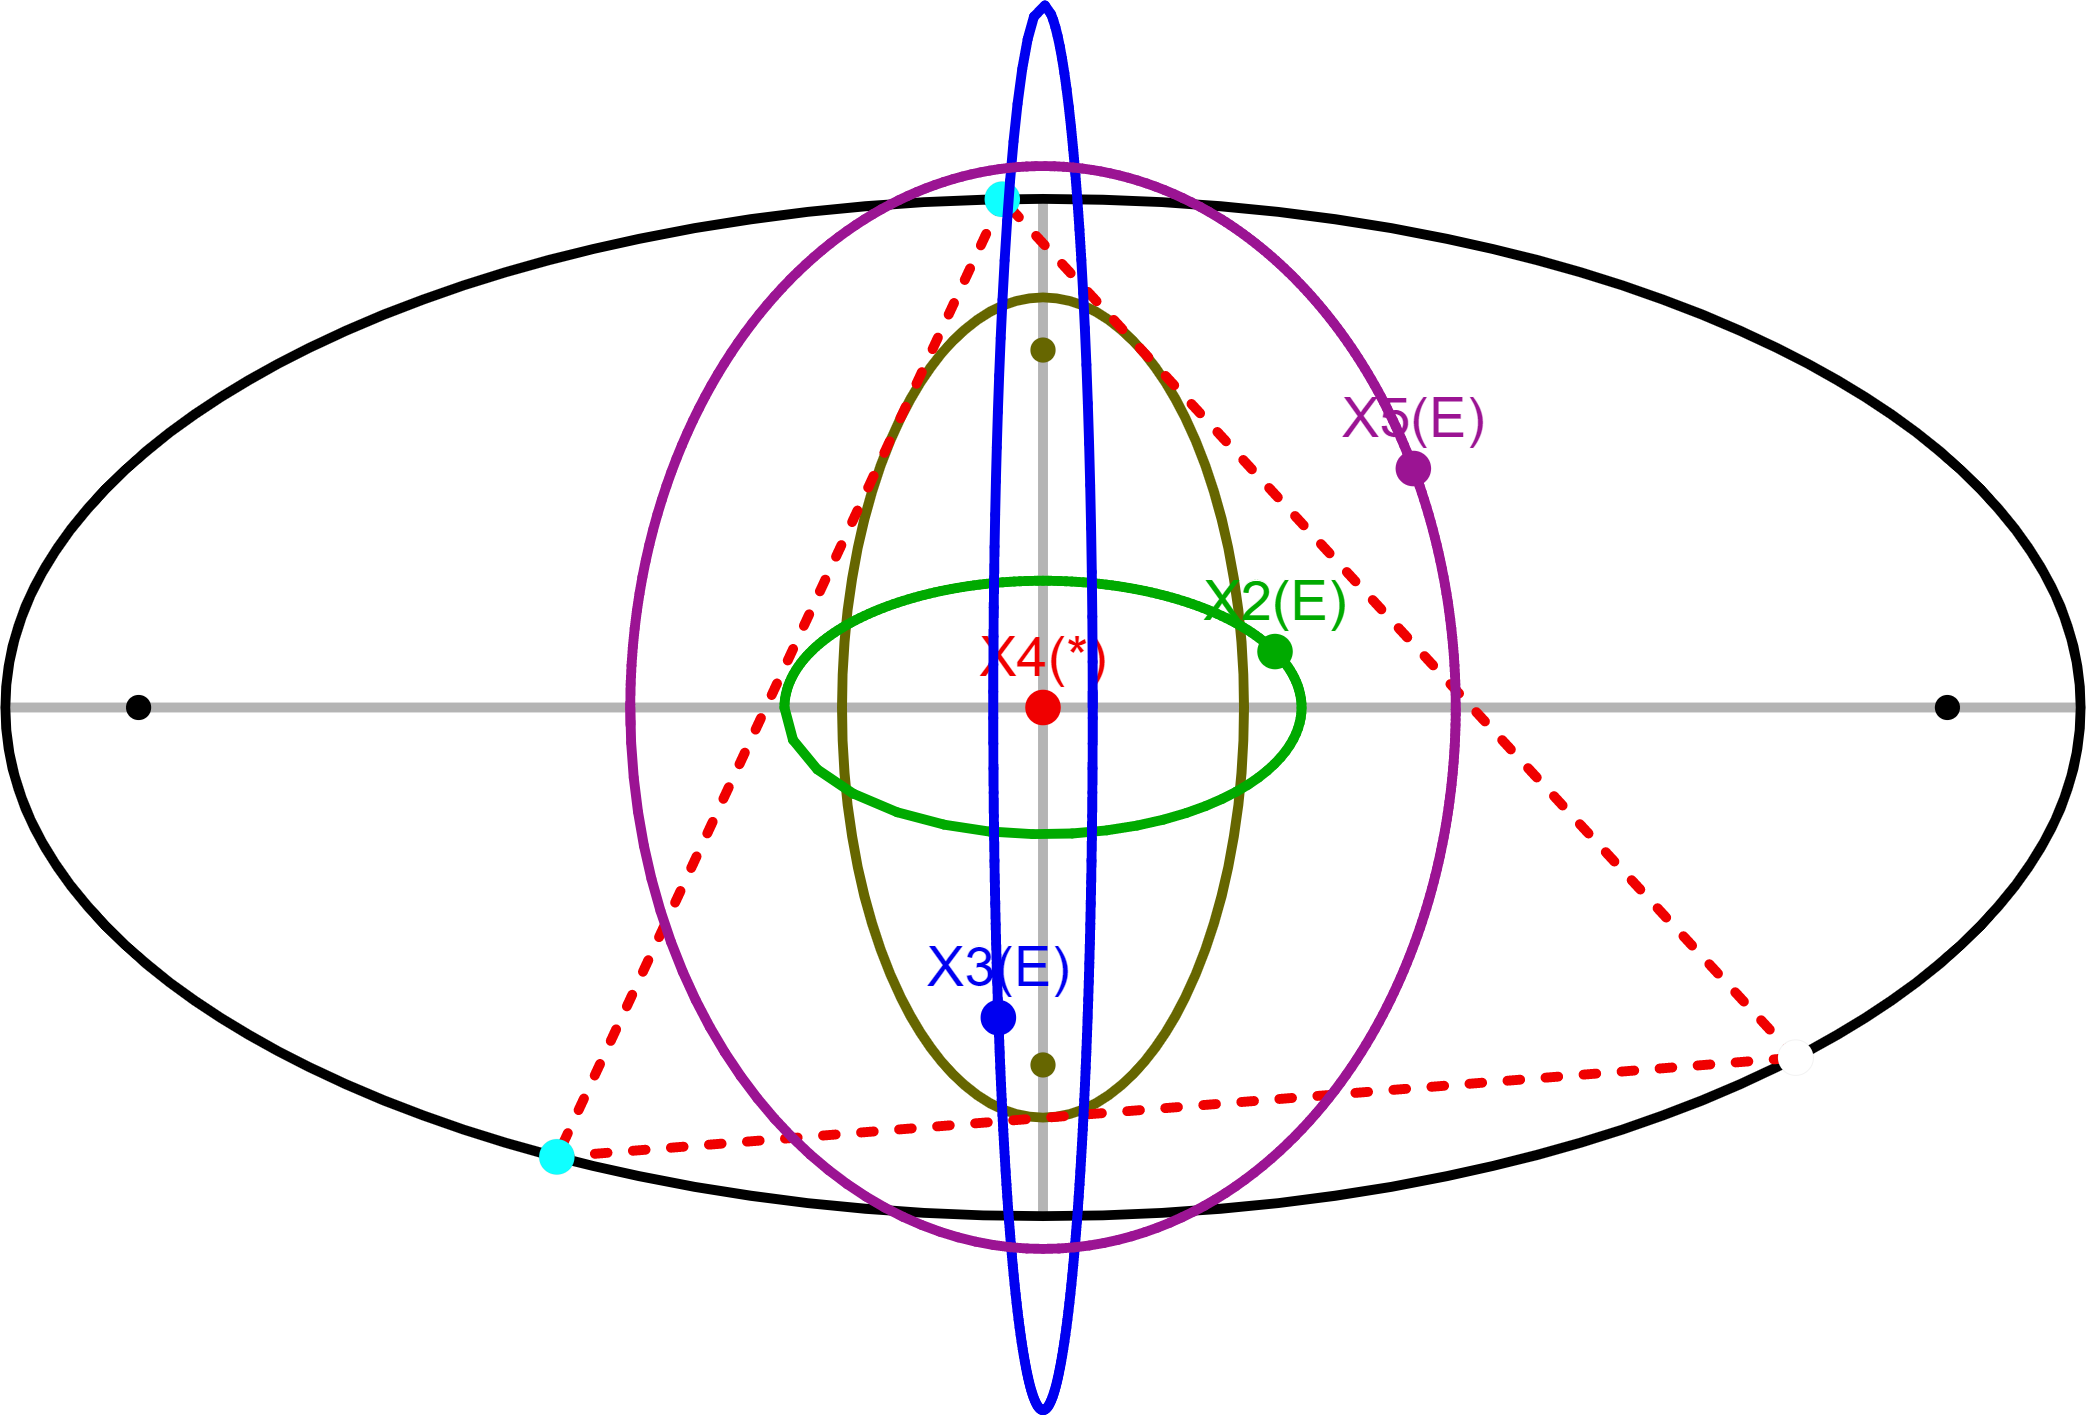
\includegraphics[width=.7\textwidth]{pics_06_100_dual_x2345.png}
    \caption{Over dual 3-periodics (stationary $X_4$), the loci of $X_2$, $X_3$, and $X_5$ are ellipses. \href{https://bit.ly/3wE3zQg}{Live}}
    \label{fig:06-dual-x2345}
\end{figure}

\section{Excentral Family}

Recall in \cref{thm:02-incenter-excenter}, we derived the semi-axes of the locus of the excenters, i.e., the ellipse in which the excentral family is inscribed. 

Also recall \cref{sec:05-golden-locus} where it was noted that over the excentral family, the locus its circumcenter ($X_{40}$ in terms of billiard 3-periodics) was identical to a rotated copy of caustic (i.e., the elliptic billiard) when the latter's aspect ratio is $\varphi$ the golden ratio.

Referring to \cref{fig:06-excentral-loci}:

\begin{proposition}
Over excentral 3-periodics the locus of $X_2$, $X_3$ and $X_4$ are ellipses.
\label{prop:06-excentral-loci}
\end{proposition}

\begin{figure}
    \centering
    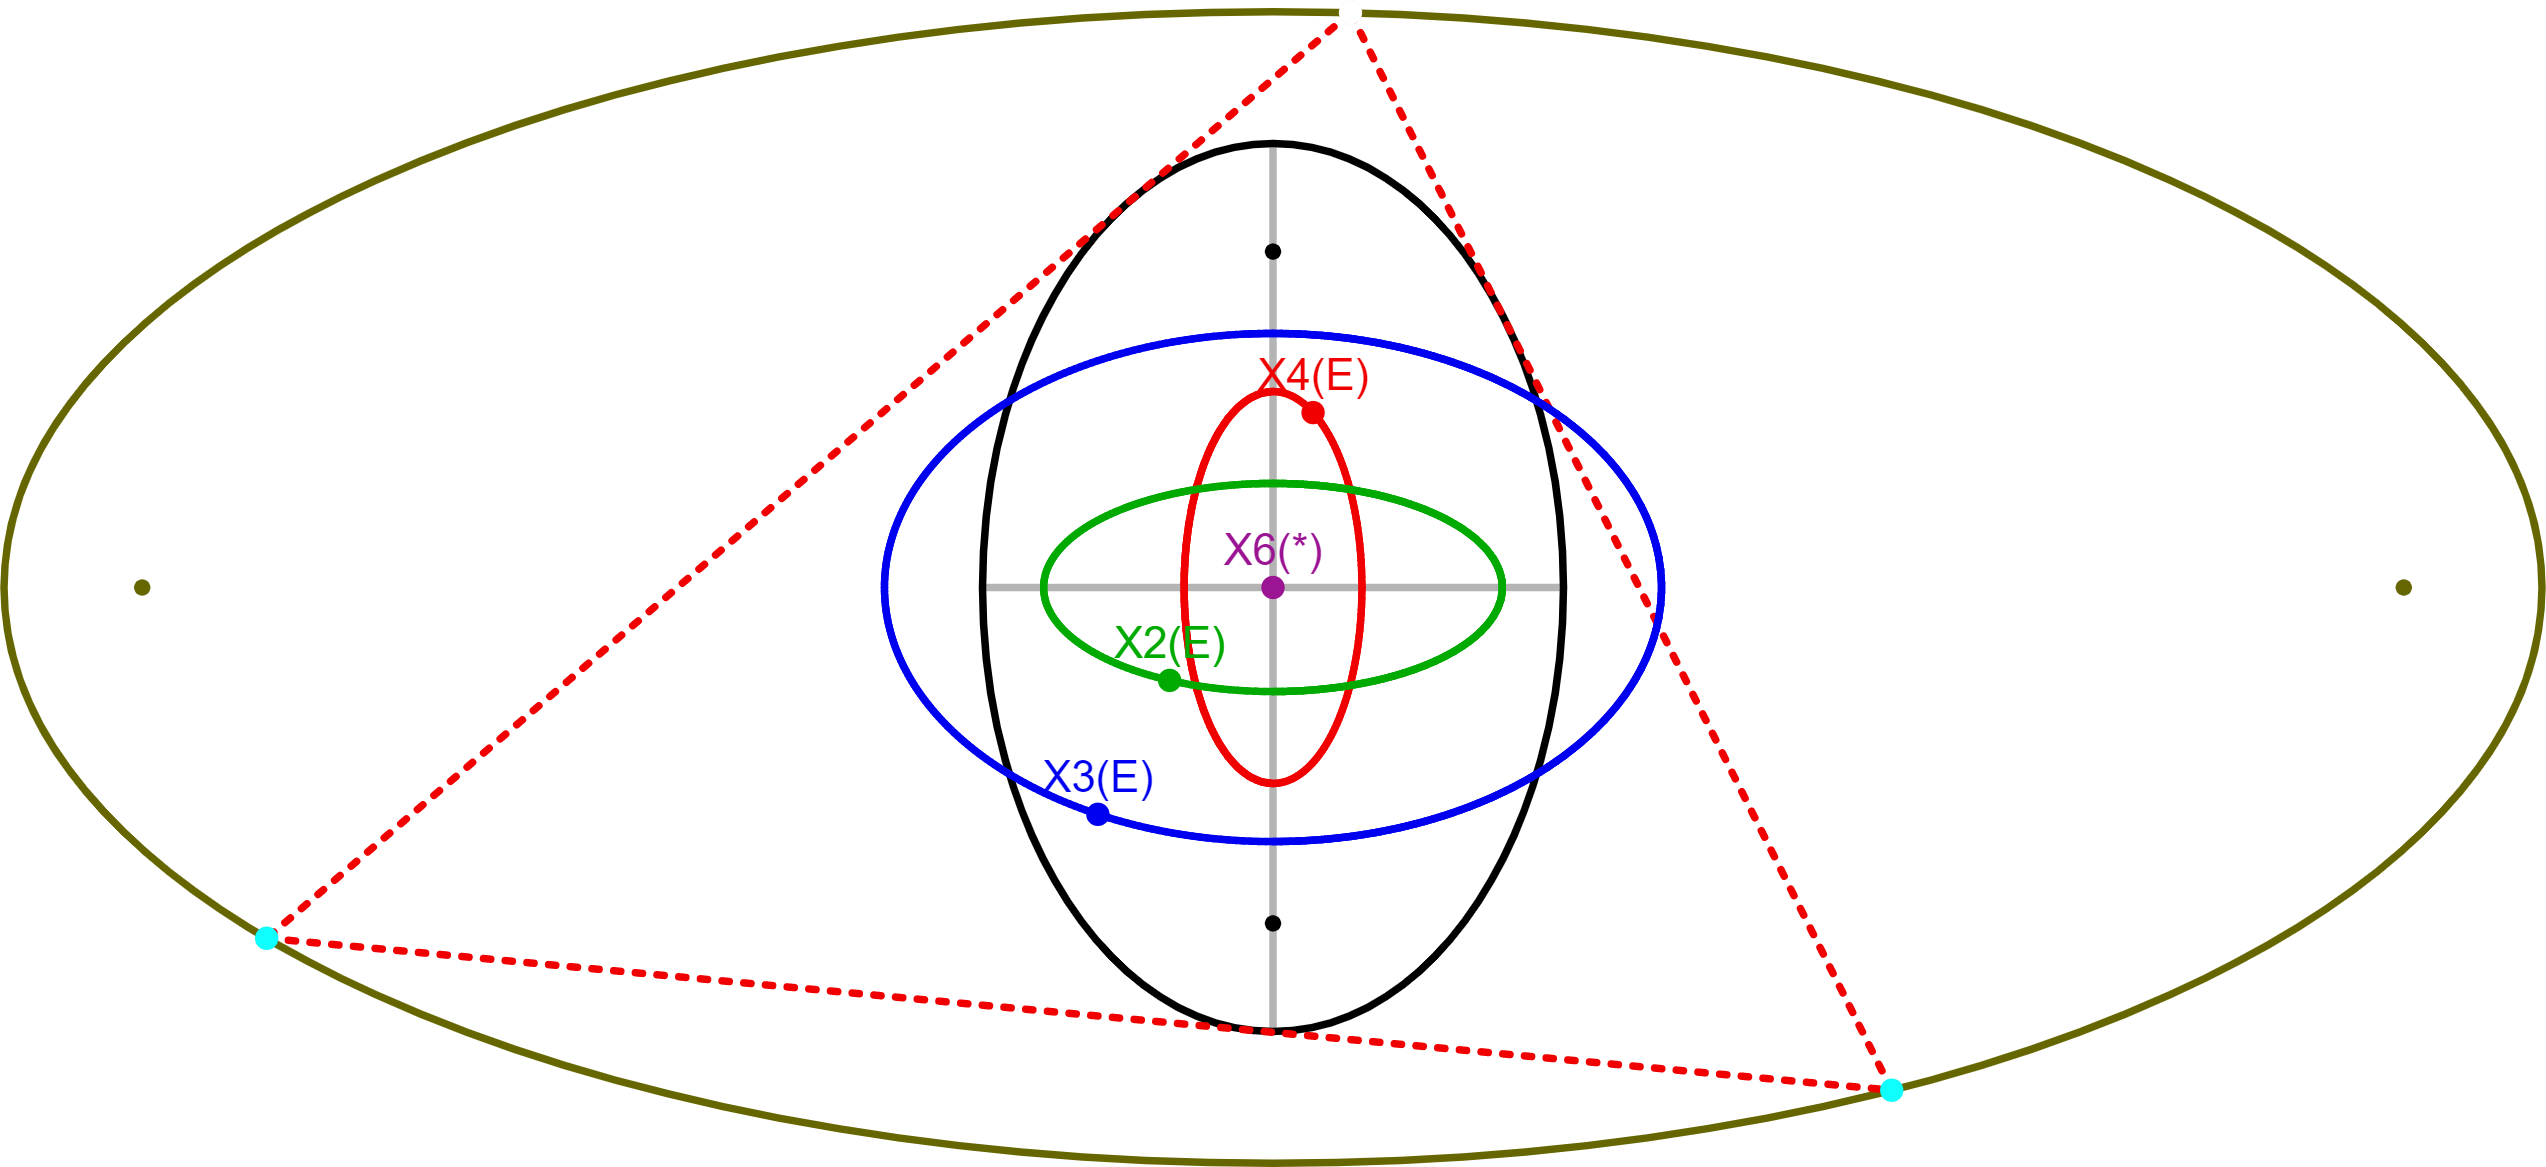
\includegraphics[width=\textwidth]{pics_06_110_excentral_loci.png}
    \caption{Elliptic loci of $X_k$, $k=$2,3,4 over excentral 3-periodics (the symmedian $X_6$ is stationary at the center). \href{https://bit.ly/2RSwAZF}{Live}}
    \label{fig:06-excentral-loci}
\end{figure}
